
\iffalse
%%%%%%%%%%%%%%%%%%%%%%%%%%%%%%%%%%%%%%%%%%%%%%%%%%%%%%%%%%%%%%%%%%%%%%%%
%
% This is the template file for the 6th International conference
% NONLINEAR ANALYSIS AND EXTREMAL PROBLEMS
% June 25-30, 2018
% Irkutsk, Russia
%
%%%%%%%%%%%%%%%%%%%%%%%%%%%%%%%%%%%%%%%%%%%%%%%%%%%%%%%%%%%%%%%%%%%%%%%%
% The preparation of the article is based on the standard llncs class
% (Lecture Notes in Computer Sciences), which is adjusted with style
% file of the conference.
%
% There are two ways of compilation of the file into PDF
% 1. Use pdfLaTeX (pdflatex), (LaTeX+DVIPS will not work);
% 2. Use LuaLaTeX (XeLaTeX will work too).
% When using LuaLaTeX You will need TTF or OTF CMU fonts
% (Computer Modern Unicode). The fonts are installed with 'cm-unicode' package in
% a distribution of LaTeX % (https://www.ctan.org/tex-archive/fonts/cm-unicode),
% either by downloading and installing these fonts system wide, the address of their page is
% http://canopus.iacp.dvo.ru/%7Epanov/cm-unicode/
% The second option won't work in XeLaTeX.
%
% For MiKTeX (LaTeX distribution for Windows),
%  1. Package 'cm-unicode' is installed manually with the MiKTeX administration Console.
%  2. For the compilation of this example, namely, the stub figure, one will also need to
% download package 'pgf' manually. This package uses in the popular
% package tikz.
%  3. Tests showed that the rest of the required packages MiKTeX loads automatically (if
%     it is allowed). The 'auto download' option is
%     configured in 'Settings' section in MiKTeX Console.
%
%
% The easiest way to compile an article is to use pdfLaTeX, but
% the final layout of the book will be compiled with LuaLaTeX,
% as a result will be of better quality thanks to the package 'microtype' and
% use vector OTF instead of standard raster fonts of pdfLaTeX.
%
% In the case of questions and problems with the article compilation,
% write letters to e-mail: eugeneai@irnok.net, Cherkashin Evgeny.
%
% New version of the correcting style file will be available at the website:
%     https://github.com/eugeneai/nla-style
%     file - nla.sty
%
% Further instructions are in the text body of the template. The template itself
% is an article example.
%
% The LaTeX2e format is used!

% 12 points font size is used.
\documentclass[12pt]{llncs}

% The correcting style file is added.
\usepackage{todonotes}

\usepackage{nla} % This package is needed for compiling
                 % this template, it should be removed
                 % from your article.

% Many popular packages (amsXXX, graphicx, etc.) are already imported in the style file.
% If there is a conflict with your packages, try disabling them and compile
% the text.
%
% It would be convenient in the layout of the proceedings if the file names
% of the figures of different authors do not clash.
% To minimize the clash, the drawings can be placed in a separate subfolder
% named after the author or the title of the paper.
%
% \graphicspath{{ivanov-petrov-pics/}} % specifies the folder with images in png, pdf formats.
% or
% \graphicspath{{great-problem-solving-paper-pics/}}.

\begin{document}
\fi
% Text should be formatted in accordance with the 'article' class, using extensions like
% AMS.
%
\title{Homogenization modeling of effective permeability for generalized Newtonian flow in porous 
media\thanks{The research is supported by the ``China Postdoctoral Science Foundation'', project No.~2023M740468,
the ``Natural Science Foundation of Liaoning Province in China'', project No.~2022-BS-093, and
the ``Education Basic Research Project of Liaoning Province in China'', project No.~JYTQN2023042.}}
% First author
\author{Shuguang Li\inst{1} \and Longjie Lv\inst{2} \and Xiaoyi Ma\inst{3}
}
\institute{School of Science, Dalian Maritime University, Dalian, 116026, China\\
  \email{lishuguang@dlmu.edu.cn}
  \and
School of Science, Dalian Maritime University, Dalian, 116026, China\\
\email{1783572186@qq.com}
\and
School of Science, Dalian Maritime University, Dalian, 116026, China\\
\email{2145297910@qq.com}}
% etc

\maketitle

\begin{abstract}
This report focuses on pore-scale modeling of generalized Newtonian fluid flow in porous media using asymptotic homogenization methods.
Local problems on periodic cells are derived to describe the local transport of generalized Newtonian fluids in pores.
The permeability tensor of generalized Newtonian fluids is obtained based on the theoretical analysis of local problems and is proved to be symmetric and positive definite.
A least squares finite element numerical solution of the local problem is developed with the help of the physical properties of the microscopic pore structure.
Solving the local problem determines the accurate distribution of velocity, pressure, and non-Newtonian viscosity in a single pore, as well as evaluating the permeability coefficient and effective viscosity.
Simulation results of Carreau-Yasuda fluid microflow in three-dimensional porous ceramics validate the proposed mathematical model and numerical method.

\keywords{Homogenization method, A generalized Newtonian fluid, Porous media, Least squares finite element method}
\end{abstract}

% at the end of the list, there should be no final dot
\section{The main results}


The non-Newtonian flow in porous medium has attracted much attention due to its important role in composite materials and petroleum industry.
However, due to the spatial multi-scale of porous medium and the rheological properties of fluids, this flow mechanism is very complex.
In this study, the asymptotic homogenization method is applied to pore-scale modeling of generalized Newtonian fluid flow in porous media.
Local problems on periodic cells are derived to describe the local transport of generalized Newtonian fluids in pores.
Based on the theoretical analysis of local problems, the permeability tensor of generalized Newtonian fluid is obtained and proved to be symmetric and positive definite, as shown in Theorem 1 below:

\textbf{Theorem 1.}
\textsl{The solution $V_{i}^{(j)}$ of the local problem has the following
relationship with the local problem:
\begin{equation*}
\displaystyle \langle v_{i}^{(0)}\rangle = K_{i}^{j}
\frac{g_{j}-p_{,x_{j}}^{(0)}}{|g_{j}-p_{,x_{j}}^{(0)}|},
\end{equation*}
where $K_{i}^{j}=\int_{\Omega_{yf}}V_{i}^{(j)}d\mathbf{y}$ is the permeability tensor
and $K_{i}^{j}$ is symmetric positive definite.
Since $V_{i}^{(j)}(\mathbf{y},|g_{j}-p^{(0)}_{,x_{j}}|)$ are nonlinear vector functions,
in fact the tensor $K_{i}^{j}(|g_{j}-p^{(0)}_{,x_{j}}|)$ is is
a symmetric positive definite tensor composed of nonlinear tensor functions.}

A least squares finite element numerical solution for local problems has been developed based on the physical properties of microscopic pore structures.
The solution of local problems can not only determine the accurate distribution of velocity, pressure and non Newtonian viscosity in a single hole, but also evaluate the permeability coefficient and effective viscosity of generalized Newtonian fluid in porous medium.
The micro flow of Carreau-Yasuda fluid in three-dimensional porous ceramics was simulated, and the proposed mathematical model and numerical method were validated.
\begin{figure}[htp]
\centering
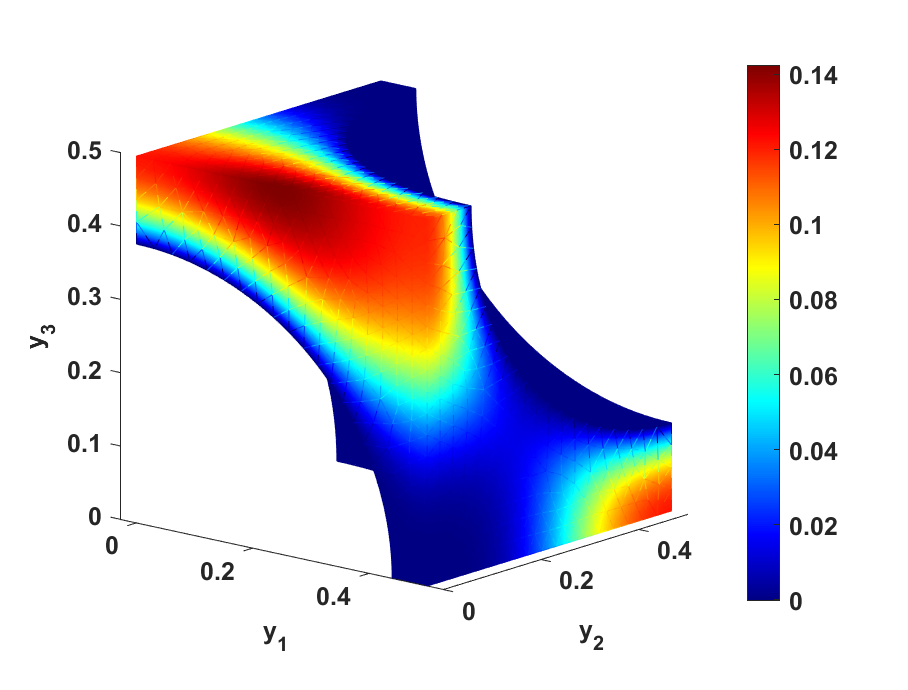
\includegraphics[width=4.1cm,height=3.9cm]{1_1.eps}
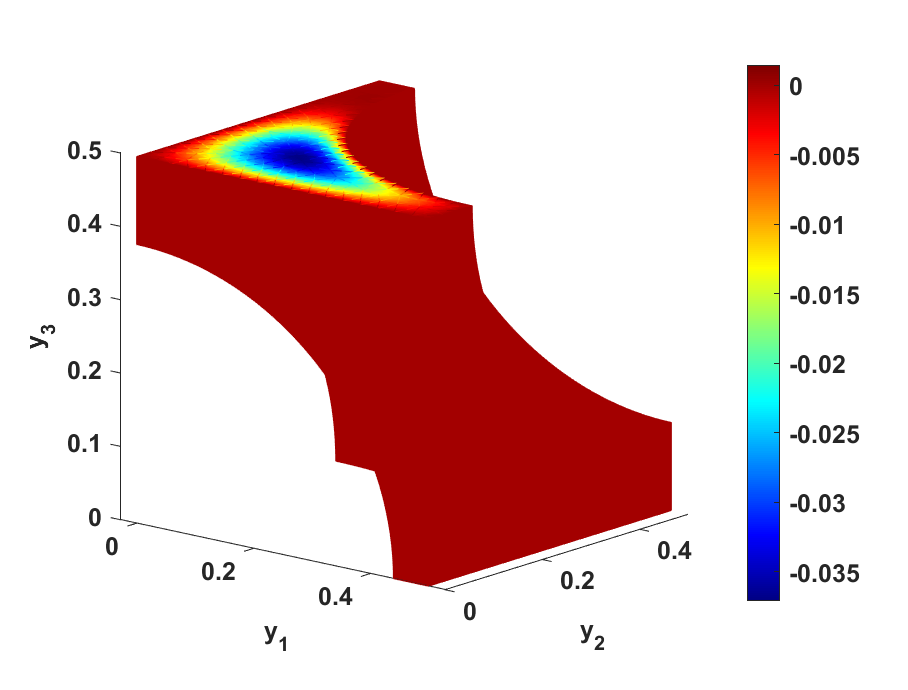
\includegraphics[width=4.1cm,height=3.9cm]{1_2.eps}
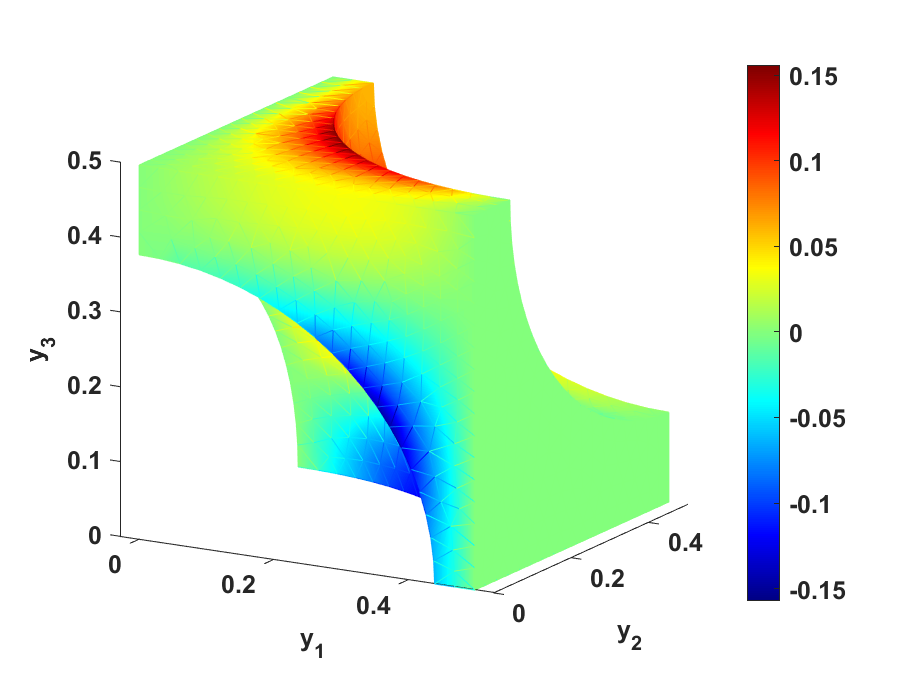
\includegraphics[width=4.1cm,height=3.9cm]{1_3.eps}
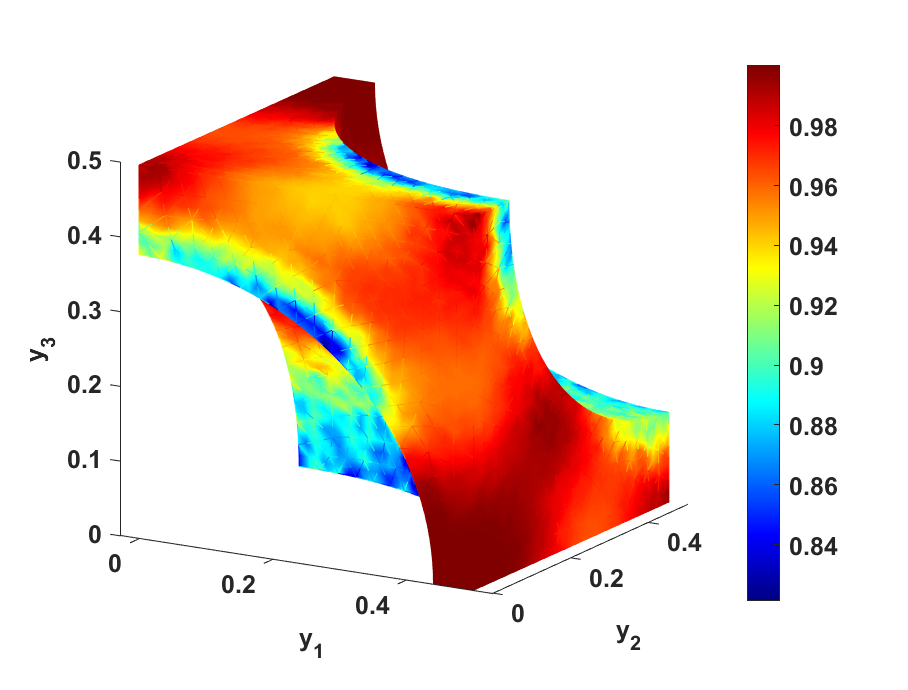
\includegraphics[width=4.1cm,height=3.9cm]{1_4.eps}\\
$(a)$\ velocity $\tilde{V}_{1}^{(1)}$\quad
$(b)$\ velocity $\tilde{V}_{2}^{(1)}$\quad
$(c)$\ pressure pulse $\tilde{P}^{(1)}$\quad
$(d)$\ non-Newtonian viscosity $\tilde{\mu}^{(1)}$\\
\small{Figure 1. Numerical results for a local problem of Carreau-Yasuda fluid in 1/8 periodic cells.}
\end{figure}

The sensitivity of non Newtonian viscosity to permeability and effective viscosity was discussed through numerical simulation.
\begin{figure}[htp]
\centering
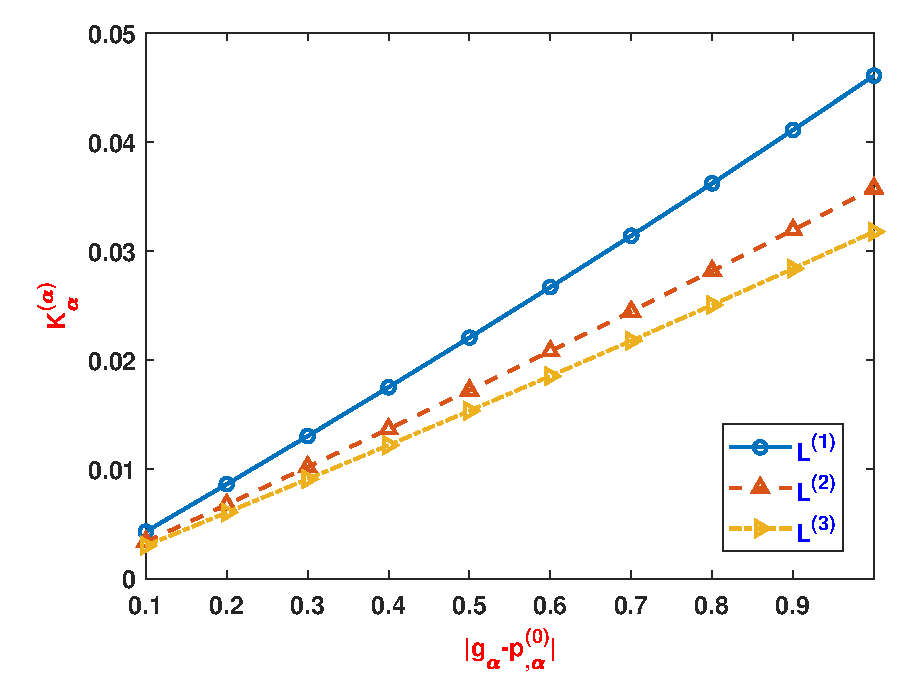
\includegraphics[width=6.4cm,height=4.2cm]{2_1.eps}
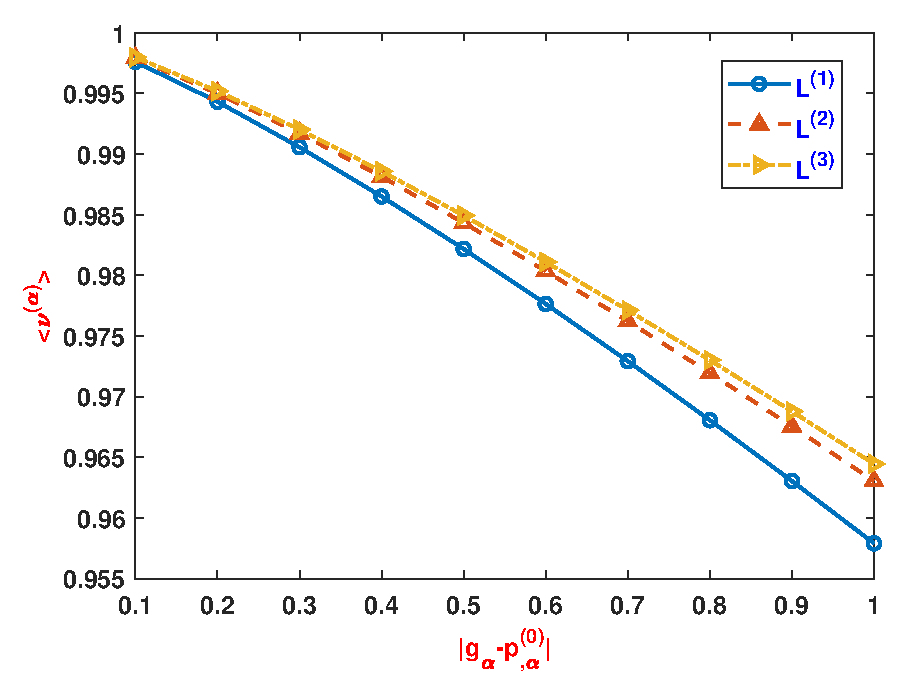
\includegraphics[width=6.4cm,height=4.2cm]{2_2.eps}\\
$(a)$\ changes in permeability tensor $K_{\alpha}^{\alpha}$\quad\quad\quad
$(b)$\ changes in effective viscosity $\mu^{(\alpha)}$\\
\small{Figure 2. The relationships between the permeability tensor $K_{\alpha}^{\alpha}$
and effective viscosity $\mu^{(\alpha)}$  of a Carreau-Yasuda fluid.}
\end{figure}

% The figures and tables are drawn according to the standard class 'article'.

\begin{thebibliography}{9} % or {99}, if there is more than ten references.
\bibitem{1} Li S.G., Dimitrienko Y.I.
    Mathematical modeling for the local flow of a generalized Newtonian fluid in 3D porous media.
    Appl. Math. Model.~2022. Vol.~105, Pp.~551--565. %https://doi.org/10.1016/j.apm.2022.01.003

\bibitem{2} Li S.G., Dimitrienko Y.I.
    Least squares finite element simulation of local transfer for a generalized Newtonian fluid in 2D periodic porous media.
    J. Non-Newton. Fluid Mech.~2023. Vol.~316, Pp.~105032. %https://doi.org/10.1016/j.jnnfm.2023.105032

\bibitem{3} Li S.G., Lv L.J., Liao M.Y. Numerical simulation of heat transfer and entropy generation due to the nanofluid natural convection with viscous dissipation in an inclined square cavity. Numer. Heat Transf. A Appl.~2024. %https://doi.org/10.1080/10407782.2024.2325121
\end{thebibliography}
%\end{document}
